\chapter*{Практика 1. Знаковое кодирование}
\addcontentsline{toc}{chapter}{Практика 1. Знаковое кодирование}
\label{ch:1_practice}
\label{sec:fig}
    

{ \itshape
    \textbf{Задание:} Реализовать знаковое кодирование и декодирование текстового сообщения.
}    
\begin{figure}[ht]
    \centering
    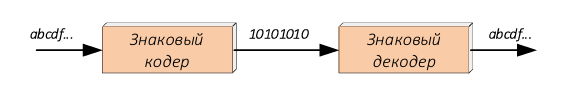
\includegraphics[width=0.8\textwidth]{symbolic_encoder_decoder.png}
    \caption{Блоксхема работы знакового кодера и декодера}
    \label{fig:symbolic_encoder_decoder.png}
\end{figure}

{
    \textbf{}

}
\begin{figure}[ht]
    \centering
    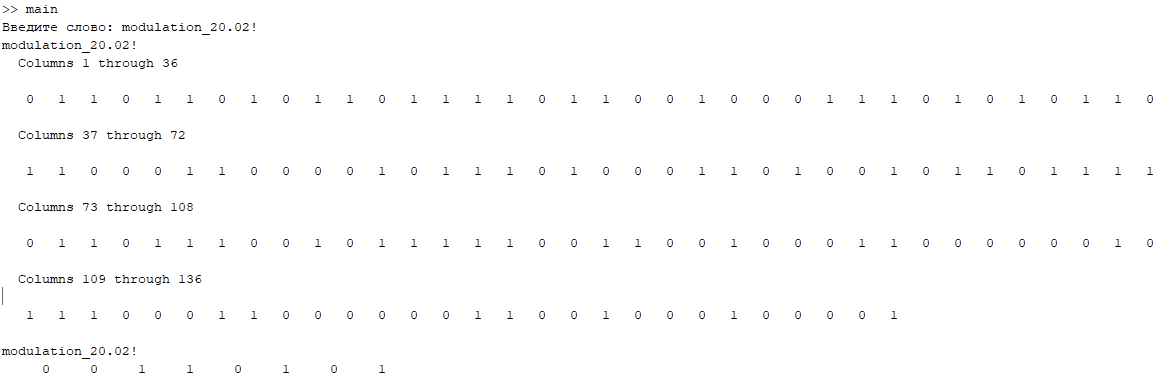
\includegraphics[width=0.8\textwidth]{1practice_result.png}
    \caption{Результат первой практики}
    \label{fig:1practice_result.png}
\end{figure}

\endinput